\begin{frame}[fragile, shrink=50]
  \frametitle{Goal-oriented adaptivity saves time}
     \vspace{-2mm}
     \begin{center}
     \begin{tikzpicture}
        \node at (8, 0) {\includegraphics[width=0.8\textwidth]{/home/meg/presentations/slides/png/flow.png}};
        \node at (0, 1) {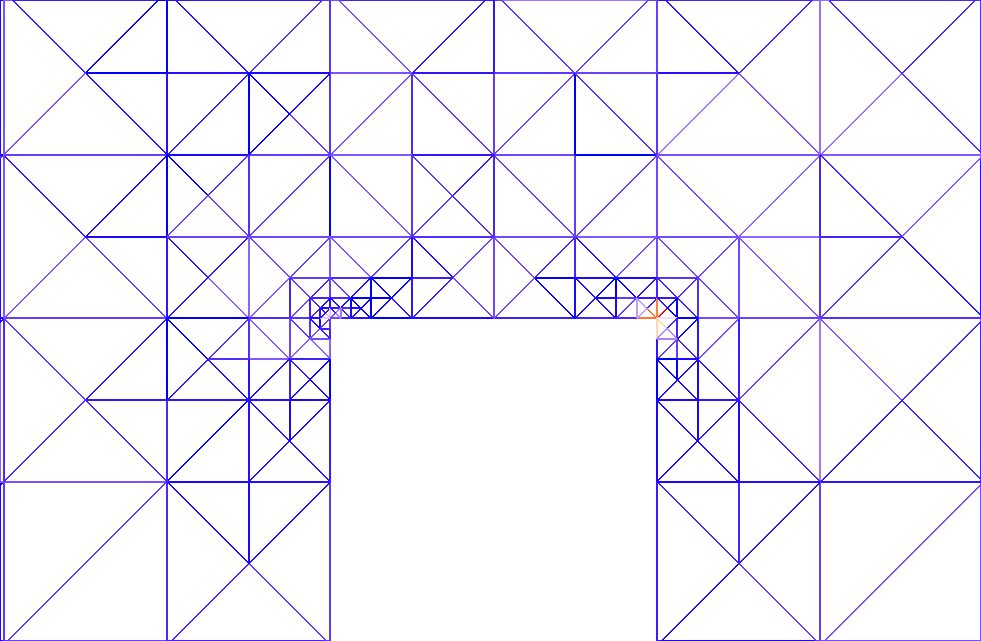
\includegraphics[width=0.3\textwidth]{/home/meg/presentations/slides/png/flow_zoom.png}};
      \end{tikzpicture}
     \end{center}
     \vspace{-8mm}
  \begin{columns}
  \vspace{-10mm}
    \begin{column}{0.4\textwidth}
      { \huge
      %\vspace{-200mm}
        Outflux $\approx 0.4087 \pm 10^{-4}$
      \begin{block}{Uniform}
        $1.000.000$ dofs, $> 3$ hours
      \end{block}
      \begin{block}{Adaptive}
        $5.200$ dofs, $31$ seconds
      \end{block}
      }
\end{column}
\begin{column}{0.6\textwidth}
  \vspace{-12mm}
  \begin{python}
from fenics import *

class Noslip(SubDomain): ...

mesh = Mesh("channel-with-flap.xml.gz"
V = VectorFunctionSpace(mesh, "Lagrange", 2)
Q = FunctionSpace(mesh, "Lagrange", 1)

# Define test functions and unknown(s)
(v, q) = TestFunctions(V * Q)
w = Function(V * Q)
(u, p) = (as_vector((w[0], w[1])), w[2])

# Define (non-linear) form
n = FacetNormal(mesh)
p0 = Expression("(4.0 - x[0])/4.0", degree=1)
F = (0.02*inner(grad(v), grad(u)) + inner(v, grad(u)*u))*dx
    - div(v)*p + q*div(u) + p0*dot(v, n)*ds
bcs = ...

# Define goal (outflux)
M = u[0]*ds(0)

# Solve!
solve(F == 0, w, bcs, tol=1.0e-4, M=M)
  \end{python}
\end{column}
\end{columns}

\end{frame}
